% !TEX program = xelatex

\documentclass{article}
\usepackage[utf8]{inputenc}
\usepackage[T1]{fontenc}
\usepackage{lmodern}
\usepackage[czech]{babel}
\usepackage[top = 1.5cm, bottom = 1.5cm, left = 2cm, right = 2cm]{geometry}
\usepackage{amsmath}
\usepackage{amssymb}
\usepackage{mathtools}
\usepackage{letltxmacro}
\usepackage{bbm}

\LetLtxMacro{\oldhbar}{\hbar}
\renewcommand*{\hbar}{{\mathpalette\hbaraux\relax\mathrm{h}}}
\newcommand*{\hbaraux}[2]{\sbox0{\mathsurround=0pt$#1\mathchar'26$}\mkern-1mu\lower.07\ht0\box0\mkern-8mu}

\def\ph{\phantom}
\def\vph{\vphantom}
\def\hph{\hphantom}
\def\rzw{\mathrlap}
\def\lzw{\mathllap}
\def\czw{\mathclap}

\newcommand{\comm}[2]{\left[ #1, #2 \right]}
\newcommand{\const}[1]{\text{#1}}
\newcommand{\norm}[1]{\left\lVert#1\right\rVert}
\newcommand{\innerprod}[2]{\big< #1, #2 \big>}
\newcommand{\mean}[1]{\left< #1 \right>}
\renewcommand{\d}[1]{\;\const{d}#1}
\newcommand{\dd}[2]{\frac{\const{d} #1}{\const{d} #2} \;}
\newcommand{\pd}[2]{\frac{\partial  #1}{\partial  #2} \;}
\newcommand{\e}[1]{\const{e}^{#1}}
\renewcommand{\i}{\const{i}}
\newcommand{\bhat}[1]{\hat{\bm{#1}}}
\newcommand{\vechat}[1]{\hat{\vec{#1}}}
\renewcommand{\dot}[1]{\accentset{\bullet}{#1}}
\newcommand{\Tr}{\operatorname{Tr}}
\newcommand{\bra}[1]{\left< #1 \right|}
\newcommand{\ket}[1]{\left| #1 \right>}
\newcommand{\braket}[2]{\left< #1 \middle| #2 \right>}
\newcommand{\f}{\varphi}
\newcommand{\Parity}{\hat{\mathcal{P}}}
\newcommand{\R}{\mathbb{R}}
\newcommand{\C}{\mathbb{C}}

\newcommand{\mat}[1]{
    \begin{pmatrix}
        #1
    \end{pmatrix}
}

\newcommand{\mata}[2]{
    \left(
    \begin{array}{@{}#1@{}}
        #2
    \end{array}
    \right)
}

\newcommand{\smat}[2][1]{
    \scalebox{#1}{$\mat{#2}$}
}

\begin{document}

\section*{Úkol 1: Kvantové tečky}
\textbf{Autor: Michal Grňo}

\subsection*{Zadání}
Máme čtyřhladinový systém s bází $\ket{A}, \ket{B}, \ket{C}, \ket{D}$ s hamiltoniánem, jehož vyjádření v této bázi je
\begin{align*}
    [ \hat H ]_{A,B,C,D}
    =
    \mat{
        \alpha & \beta & \gamma & \beta \\
        \beta & \alpha & \beta & \gamma \\
        \gamma & \beta & \alpha & \beta \\
        \beta & \gamma & \beta & \alpha
    } \: ,
    \quad
    \alpha, \beta, \gamma \in \R \: .
\end{align*}
Tento systém odpovídá čtyřem kvantovým tečkám. Definujeme operátory souřadnic a zrcadlení:
\begin{align*}
    \hat X &= \ket{A}\bra{A} - \ket{C}\bra{C}, &
    \hat Y &= \ket{B}\bra{B} - \ket{D}\bra{D}, \\
    \Parity_\const{X} &= \ket{A}\bra{C} + \ket{C}\bra{A}, &
    \Parity_\const{Y} &= \ket{B}\bra{D} + \ket{D}\bra{B}.
\end{align*}
Najděte eigenbázi operátorů $\Parity_\const{X}, \Parity_\const{Y}$, v ní vyjádřete $\hat H$ a následně ho diagonalizujte. Dále si představte, že máme systém ve stavu $X=0, Y=1$ a $\hat H$ – jaké jsou pravděpodobnosti naměření jednotlivých energetických hladin?

\subsection*{Řešení}
Začneme nalezením eigenbáze $\Parity_\const{X}, \Parity_\const{Y}$. Vidíme, že každý z těchto operátorů je netriviální pouze na dvourozměrném podprostoru. Toho využijeme.
\begin{align*}
    [\Parity_\const{X}]_{A,C} &= \smat[0.8]{0 & 1 \\ 1 & 0}, &
    [\Parity_\const{Y}]_{B,D} &= \smat[0.8]{0 & 1 \\ 1 & 0}. &
    \smat[0.8]{0 & 1 \\ 1 & 0} \; &\sim \;
    1 \cdot \smat[0.8]{1 \\ 1}, \;\; -1 \cdot \smat[0.8]{\ph{-}1 \\ -1}
\end{align*}
Hledaná báze je tedy $\big\{ \frac{1}{\sqrt{2}}( \ket{A}+\ket{C} ), \; \frac{1}{\sqrt{2}}( \ket{A}-\ket{C} ), \; \frac{1}{\sqrt{2}}( \ket{B}+\ket{D} ), \; \frac{1}{\sqrt{2}}( \ket{B}-\ket{D} ) \big\} \eqqcolon \big\{ \ket{a}, \ket{b}, \ket{c}, \ket{d} \big\}$. Vlastní čísla operátoru $\Parity_\const{X}$ jsou potom $+1, -1, 0, 0$ a vlastní čísla $\Parity_\const{Y}$ jsou $0, 0, +1, -1$. Vyjádříme si matici přechodu:
\begin{align*}
    R &= [\mathbbm{1}]^{A,B,C,D}_{a,b,c,d} =
    \frac{1}{\sqrt{2}}
    \smat[0.9]{
        1 & 1 & 0 & 0 \\
        0 & 0 & 1 & 1 \\
        1 &\!-1 & 0 & 0 \\
        0 & 0 & 1 &\!-1
    } \: ,
    &
    R^{-1} = R^T =
    \frac{1}{\sqrt{2}}
    \smat[0.9]{
        1 & 0 & 1 & 0 \\
        1 & 0 &\!-1 & 0 \\
        0 & 1 & 0 & 1 \\
        0 & 1 & 0 &\!-1
    } \: .
\end{align*}
\begin{align*}
    [\hat H]_{a,b,c,d} = R^{-1} \; [\hat H]_{A,B,C,D} \; R
    =
    \frac{1}{2}
    \smat[0.9]{
        1 &   & 1 &   \\
        1 &   &\lzw{-}1 & \\
          & 1 &   & 1 \\
          & 1 &   &\lzw{-}1
    }
    \smat[0.9]{
        \alpha & \beta & \gamma & \beta \\
        \beta & \alpha & \beta & \gamma \\
        \gamma & \beta & \alpha & \beta \\
        \beta & \gamma & \beta & \alpha
    }
    \smat[0.9]{
        1 & 1 &   &   \\
          &   & 1 & 1 \\
        1 &\!-1 &   & \\
          &   & 1 &\!-1
    }
    =
    \smat[0.9]{
        \alpha + \gamma \! & & 2\beta \\
        & \! \alpha - \gamma \! \\
        2\beta & & \! \alpha + \gamma \! \\
        & & & \! \alpha - \gamma
    } \: .
\end{align*}
Vidíme, že prohozením prvků báze $\ket{b} \!\leftrightarrow\! \ket{c}$ získáme blokově diagonální matici:
\begin{align*}
    [\hat H]_{a,c,b,d} =
    \smat[0.9]{
        \alpha + \gamma  & 2\beta \\
        2\beta &  \alpha + \gamma \! \\
        & &\! \alpha - \gamma \! \\
        & & & \! \alpha - \gamma
    }
\end{align*}
Zjevně $\ket{b}$ a $\ket{d}$ už jsou vlastními vektory s vlastní hodnotou $\alpha - \gamma$. Diagonalizujeme blok $\ket{a}, \ket{c}$:
\begin{align*}
    0 &=
    \begin{vmatrix}
        \alpha + \gamma - \lambda & 2\beta \\
        2\beta & \alpha + \gamma - \lambda
    \end{vmatrix}
    = (\alpha + \gamma - \lambda)^2 - (2\beta)^2
\end{align*}
\begin{align*}
    (2\beta)^2
    &=
    (\alpha + \gamma - \lambda)^2
    \\
    \pm 2\beta
    &=
    \alpha + \gamma - \lambda
    \\
    \lambda
    &=
    \alpha + \gamma \pm 2\beta
\end{align*}
\begin{align*}
    \lambda = \alpha + \gamma - 2\beta : \;
    &\ker \smat[0.9]{2\beta & 2\beta}
    = \mat{\ph{-}1 \\ -1}
    \\
    \lambda = \alpha + \gamma + 2\beta : \;
    &\ker \smat[0.9]{-2\beta & 2\beta}
    = \mat{1 \\ 1}
\end{align*}
Dostáváme tedy eigenbázi hamiltoniánu:
\begin{align*}
    \ket{1} &= \ket{b} = \frac{1}{\sqrt{2}} (\ket{A} - \ket{C}) \\
    \ket{2} &= \ket{d} = \frac{1}{\sqrt{2}} (\ket{B} - \ket{D}) \\
    \ket{3} &= \frac{1}{\sqrt{2}} (\ket{a} - \ket{c})
    = \frac{1}{2} (\ket{A} - \ket{B} + \ket{C} - \ket{D})\\
    \ket{4} &= \frac{1}{\sqrt{2}} (\ket{a} + \ket{c})
    = \frac{1}{2} (\ket{A} + \ket{B} + \ket{C} + \ket{D})
\end{align*}
Vlastní čísla odpovídající těmto vektorům jsou $\alpha - \gamma, \;\; \alpha - \gamma, \;\; \alpha + \gamma - 2\beta, \;\; \alpha + \gamma + 2\beta$.

Nakonec nás zajímá pravděpodobnost těchto energetických hodnot, změříme-li nejprve polohu a potom $\hat H$. Protože vlastními vektory operátorů $\hat X$ a $\hat Y$ jsou $\ket{A}, \ket{B}, \ket{C}, \ket{D}$, po změření polohy některý z těchto stavů. Naměřeným hodnotám $X=0, Y=1$ konkrétně odpovídá stav $\ket{B}$.
\begin{align*}
    P(\alpha - \gamma) = P_1 + P_2
    &= \big|\braket{B}{1}\big|^2 + \big|\braket{B}{2}\big|^2
    = \frac{1}{2}
    \\[5pt]
    P(\alpha + \gamma - 2\beta) = P_3
    &= \big|\braket{B}{3}\big|^2
    = \frac{1}{4}
    \\[5pt]
    P(\alpha + \gamma + 2\beta) = P_4
    &= \big|\braket{B}{4}\big|^2
    = \frac{1}{4}
\end{align*}
Tedy máme 50\% šanci, že naměříme degenerovanou hladinu $\alpha - \gamma$, a zbylé dvě nedegenerované hladiny mají po~25~\%.

\subsection*{Zábavný dodatek}
Výňatek z abstraktu publikace \textit{A strong no-go theorem on the Wigner’s friend paradox}, Bong et al., 2020:

Does quantum theory apply at all scales, including that of observers? [Here] we rigorously prove that if quantum evolution is controllable on the scale of an observer, then one of the following three assumptions must be false: "No-Superdeterminism", "Locality", or "Absoluteness of Observed Events" (i.e. that every observed event exists absolutely, not relatively). [...] We demonstrate this in a proof-of-principle experiment where \textbf{a photon's path is deemed an observer}.

\begin{figure}[h!]
    \centering
    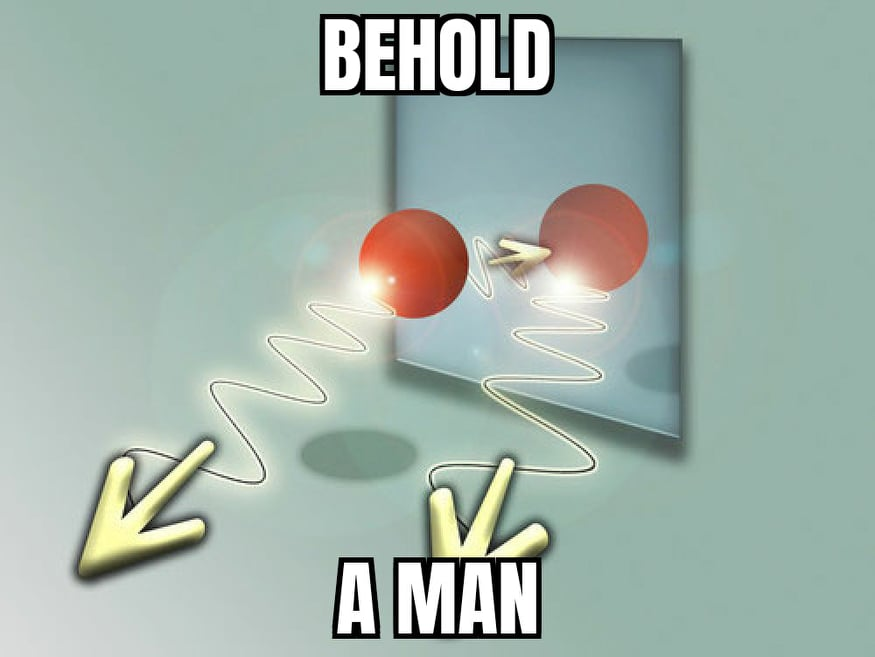
\includegraphics[width=200pt]{meme.jpg}
    \caption{Skutečná fotografie experimentu.}
  \label{fig:boat1}
\end{figure}


\end{document}
